\documentclass[12pt,letterpaper]{exam}
\usepackage[lmargin=1in,rmargin=1in,tmargin=1in,bmargin=1in]{geometry}
\usepackage{../style/exams}

% -------------------
% Course & Exam Information
% -------------------
\newcommand{\course}{MATH 122: Exam 2}
\newcommand{\term}{Fall --- 2024}
\newcommand{\examdate}{10/15/2024}
\newcommand{\timelimit}{75 Minutes}

\setbool{hideans}{false} % Student: True; Instructor: False

% -------------------
% Content
% -------------------
\begin{document}

\examtitle
\instructions{Write your name on the appropriate line on the exam cover sheet. This exam contains \numpages\ pages (including this cover page) and \numquestions\ questions. Check that you have every page of the exam. Answer the questions in the spaces provided on the question sheets. Be sure to answer every part of each question and show all your work. If you run out of room for an answer, continue on the back of the page --- being sure to indicate the problem number.} 
\scores
\bottomline
\newpage


% -------------------
% Questions
% -------------------
\begin{questions}

% Question 1
\newpage
\question[20] Consider the function $f(x)$ plotted below. 
	\[
	\fbox{
	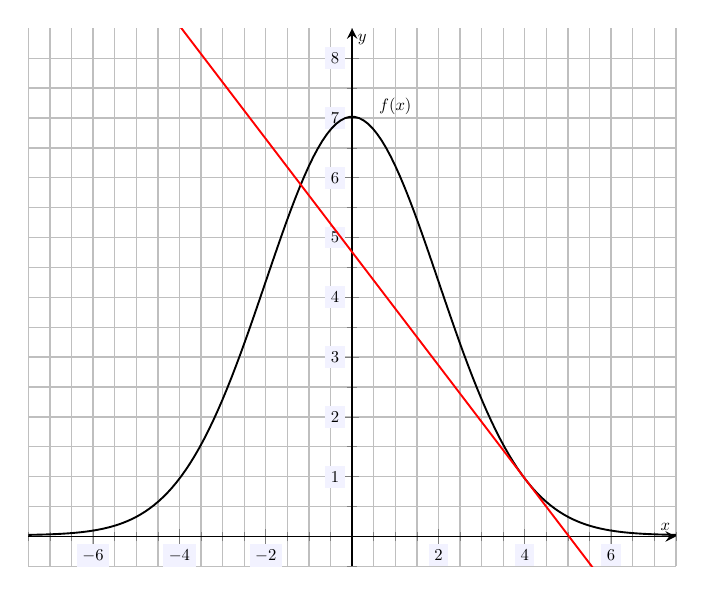
\begin{tikzpicture}[scale=1.2,every node/.style={scale=0.5}]
	\begin{axis}[
	grid=both,
	axis lines=middle,
	ticklabel style={fill=blue!5!white},
	xmin= -7.5, xmax=7.5,
	ymin= -0.5, ymax=8.5,
	xtick={-8,-6,...,8},
	ytick={-1,0,...,8},
	minor tick = {-8,-7.5,...,8},
	xlabel=\(x\),ylabel=\(y\),
	]
	\addplot[line width= 0.02cm,samples=200,domain= -10.5:10.5] ({x},{7*e^(-x^2/8) + 0.02});
	\addplot[red,line width= 0.02cm,samples=200,domain= -10.5:10.5] ({x},{-0.947*x + 4.757});
	\node at (1,7.2) {$f(x)$};
	\end{axis}
	\end{tikzpicture}
	}
	\] \par
Based on the plot above, answer the following: \par
	\begin{enumerate}[(a)]
        	\item On what interval(s)---if any---is $f'(x) > 0$? \vfill
	
	{\itshape If $f'(x) > 0$, then $f(x)$ is increasing. But then $f'(x) > 0$ on $(-\infty, 0)$.} \vfill
	
	\item On what interval(s)---if any---is $f'(x) < 0$? \vfill
	
	{\itshape If $f'(x) < 0$, then $f(x)$ is decreasing. But then $f'(x) < 0$ on $(0, \infty)$.} \vfill
	
	\item Find any points of inflection---if any. \vfill
	
	{\itshape We can see points of inflection at $x= -2$ and $x= 2$, i.e. $(-2, 4.27)$ and $(2, 4.27)$.} \vfill
	
	\item On what interval(s)---if any---is $f''(x) > 0$? \vfill
	
	{\itshape If $f''(x) > 0$, then $f$ is concave up. From (c) and the graph, this is $(-\infty, -2) \cup (2, \infty)$.} \vfill
	
	\item On what interval(s)---if any---is $f''(x) < 0$? \vfill
	
	{\itshape If $f''(x) < 0$, then $f$ is concave down. From (c) and the graph, this is $(-2, 2)$.} \vfill
	
	\item Determine whether the following are positive ($> 0$), negative ($< 0$), or zero ($= 0$): 
		\begin{2itemize}
		\item $f(-2)$ \hspace{0.1cm} \underline{\phantom{==}$>$\phantom{==}} \hspace{0.1cm} 0 
		\item $f'(0)$ \phantom{$-$} \underline{\phantom{==}$=$\phantom{==}} \hspace{0.1cm} 0
		\item $f''(5)$ \phantom{$'''$} \underline{\phantom{==}$>$\phantom{==}} \hspace{0.1cm} 0
		\item $f'(-3)$ \underline{\phantom{==}$>$\phantom{==}} \hspace{0.1cm} 0 \pvspace{0.2cm}
		\item $f'(5)$ \phantom{$.'$} \underline{\phantom{==}$<$\phantom{'....''}} \hspace{0.1cm} 0 \pvspace{0.2cm}
		\item $f''(0)$ \phantom{$l$} \underline{\phantom{==}$<$\phantom{'....''}} \hspace{0.1cm} 0
		\end{2itemize} \vfill
	\item Sketch the tangent line to $f(x)$ at $x= 4$ on the graph above. \vfill
	
	{\itshape See the drawn red line.} \vfill
	\end{enumerate}



% Question 2
\newpage
\question[15] Showing all your work, compute the derivatives given below. {\itshape Do not simplify your answer.} \pvspace{0.3cm}
	\begin{enumerate}[(a)]
	\item $\dfrac{d}{dx} \left( x^6 - 3x + \dfrac{1}{\sqrt{x}} - 11 \right)= \dfrac{d}{dx} \left( x^6 - 3x + x^{-1/2} - 11 \right)= 6x^5 - 3 - \frac{1}{2}\, x^{-3/2}$ \vfill
	
	\item $\dfrac{d}{dx} (x^{10}\, 2^x)= 10x^9 \cdot 2^x + x^{10} \cdot 2^x \ln 2$ \vfill
	
	\item $\dfrac{d}{dx}\, \ln(5x^2 - x)= \dfrac{1}{5x^2 - x} \cdot (10x - 1)$ \vfill
	
	\item $\dfrac{d}{dx} \, (5\pi^3)= 0$ \vfill
	
	\item $\dfrac{d}{dx} \left(\dfrac{6x - 1}{x^2 + 1} \right)= \dfrac{6(x^2 + 1) - 2x(6x - 1)}{(x^2 + 1)^2}$ \vfill
	\end{enumerate}



% Question 3
\newpage
\question[15] Consider the \textit{derivative} of a function, $f'(x)$, plotted below. 
	\[
	\fbox{
	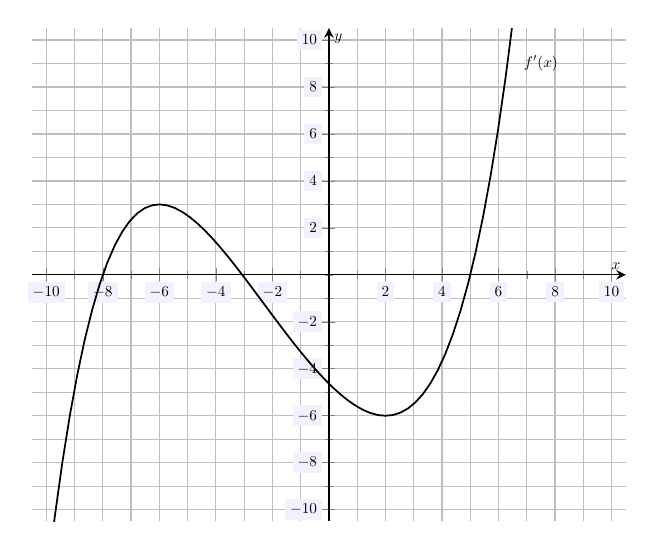
\begin{tikzpicture}[scale=1.1,every node/.style={scale=0.5}]
	\begin{axis}[
	grid=both,
	axis lines=middle,
	ticklabel style={fill=blue!5!white},
	xmin= -10.5, xmax=10.5,
	ymin= -10.5, ymax=10.5,
	xtick={-10,-8,-6,-4,-2,0,2,4,6,8,10},
	ytick={-10,-8,-6,-4,-2,0,2,4,6,8,10},
	minor tick = {-10,-9,...,10},
	xlabel=\(x\),ylabel=\(y\),
	]
	\addplot[line width= 0.02cm,samples=80,domain= -10.5:10.5] ({x},{-4.6345 - 1.19714*x + 0.18566*x^2 + 0.030597*x^3 + 0.0020121*x^4 + 0.000286889*x^5});
	\node at (7.5,9) {$f'(x)$};
	\end{axis}
	\end{tikzpicture}
	}
	\] 
Based on the plot above, answer the following questions: 
	\begin{enumerate}[(a)]
	\item On what interval(s)---if any---is $f(x)$ increasing? \vfill
	
	{\itshape\small If $f'(x) > 0$, then $f(x)$ is increasing. Therefore, $f(x)$ is increasing on $(-8, -3) \cup (5, \infty)$.} \vfill 
	
	\item On what interval(s)---if any---is $f(x)$ decreasing? \vfill
	
	{\itshape\small If $f'(x) > 0$, then $f(x)$ is decreasing. Therefore, $f(x)$ is decreasing on $(-\infty, -8) \cup (-3, 5)$.} \vfill 
	
	\item On what interval(s)---if any---is $f(x)$ concave up? \vfill
	
	{\itshape If $f(x)$ is concave up, $f''(x) > 0$. But then $f'(x)$ is increasing. Therefore, $f(x)$ is concave up on $(-\infty, -6) \cup (2, \infty)$.} \vfill 
	
	\item On what interval(s)---if any---is $f(x)$ concave down? \vfill
	
	{\itshape If $f(x)$ is concave down, $f''(x) < 0$. But then $f'(x)$ is decreasing. Therefore, $f(x)$ is concave down on $(-6, 2)$.} \vfill 
	
	\item Find any critical values for $f(x)$---if any. \vfill
	
	{\itshape The critical values are where $f'(x)= 0$. But these values are $x= -8, -3, 5$.} \vfill 
	
	\item Classify any critical values you found in (e). \vfill
	
	\phantom{.} \hfill 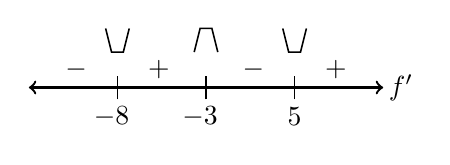
\begin{tikzpicture}[scale=0.75]
	\draw[line width=0.03cm,<->] (-3,0) -- (3,0);
	\draw[line width=0.02cm] (-1.5,-0.2) -- (-1.5,0.2);
	\draw[line width=0.02cm] (0,-0.2) -- (0,0.2);
	\draw[line width=0.02cm] (1.5,-0.2) -- (1.5,0.2);
	\node at (3.3,0) {$f'$};
	\node at (-1.6,-0.5) {$-8$};
	\node at (-0.1,-0.5) {$-3$};
	\node at (1.5,-0.5) {$5$};
	
	\node at (-2.2,0.3) {$-$};
	\node at (-0.8,0.3) {$+$};
	\node at (0.8,0.3) {$-$};
	\node at (2.2,0.3) {$+$};
	
	\draw[line width=0.02cm] (-1.7,1) -- (-1.6,0.6) -- (-1.4,0.6) -- (-1.3,1);
	\draw[line width=0.02cm] (1.3,1) -- (1.4,0.6) -- (1.6,0.6) -- (1.7,1);
	\draw[line width=0.02cm] (-0.2,0.6) -- (-0.1,1) -- (0.1,1) -- (0.2,0.6);
	\end{tikzpicture} \hfill \phantom{.}
	
	{\itshape Alternatively, we know $f''(x) > 0$ at $x= -8, 5$ and $f''(x) < 0$ at $x= -3$. Therefore, $x= -8, 5$ are minima and $x= -3$ is a maxima.} \vfill 
	
	\item Find any points of inflection for $f(x)$. \vfill
	
	{\itshape An inflection point is where $f''(x)$ changes sign. From (c) and (d), we can see this is at $x= -6, 2$.} \vfill 
	\end{enumerate}



% Question 4
\newpage
\question[15] Showing all your work, compute the derivatives given below. {\itshape Do not simplify your answer.} \pvspace{0.3cm}
	\begin{enumerate}[(a)]
	\item $\dfrac{d}{dx} (3x^2\, e^{-x}\, \log_5(x) \big)= 6x \cdot e^{-x} \log_5 x + -e^{-x} \cdot 3x^2 \log_5 x + \dfrac{1}{x \ln 5} \cdot 3x^2 e^{-x}$ \vfill
	\item $\dfrac{d}{dx} \big(9^{x^3} - x \big)^7= 7 \left( 9^{x^3} - x \right)^6 \cdot \left( 9^{x^3} \ln 9 \cdot 3x^2 - 1 \right)$ \vfill
	\item $\dfrac{d}{dx} \left( \dfrac{(3x - 1) e^{2x}}{\ln(1 - x)} \right)= \dfrac{\big( 3 \cdot e^{2x} + 2e^{2x} \cdot (3x - 1) \big) \ln(1 - x) - \left( \dfrac{1}{1 - x} \cdot -1 \right) \cdot \big( (3x - 1) e^{2x} \big)}{ \big( \ln(1 - x) \big)^2}$ \vfill
	\end{enumerate}



% Question 5
\newpage
\question[15] A company produces widgets. They hire financial analysts to examine their production costs. The analysts determine that if $q$ items are produced, then the total production cost for the widgets is given by $C(q)= 223,\!000 + 1,\!000q - q^2$. 
	\begin{enumerate}[(a)]
	\item Find the fixed costs for producing these widgets. 
	\item Find the marginal costs at a production level of $q= 180$.
	\item What level of production maximizes the total cost of producing these widgets? Be sure to justify your answer with either the first or second derivative test. 
	\end{enumerate} \pspace

{\itshape \tsol
	\begin{enumerate}[(a)]
	\item The fixed costs are the cost not associated with the production of the widgets. But these are the costs at a production level of $q= 0$. Therefore, the fixed costs are\dots
		\[
		C(0)= 223,\!000 + 1,\!000(0) - 0^2= 223,\!000 + 0 + 0= \$223,\!000
		\] \pspace
	
	\item We know the marginal costs are the (approximate) costs of producing the next item. But this cost is approximately $C'(q)$. But then the marginal costs at a production level of $q= 180$ are $C'(180)$. We have\dots
		\[
		\begin{aligned}
		C'(q)&= 1,\!000 - 2q \\[0.3cm]
		C'(180)&= 1,\!000 - 2(180)= 1,\!000 - 360= \$640 
		\end{aligned}
		\]
	Therefore, the marginal costs at a production level of $q= 180$~items is \$640. \pspace
	
	\item We know maxima or minima occur when the derivative is zero, i.e. at critical values. We know from (b) that $C'(q)= 1000 - 2q$. Setting $C'(q)= 0$, we have\dots
		\[
		\begin{gathered}
		C'(q)= 0 \\[0.3cm]
		1000 - 2q= 0 \\[0.3cm]
		2q= 1000 \\[0.3cm]
		q= 500
		\end{gathered}
		\] \par
	Using the first derivative test, we have\dots \par
		\[
        		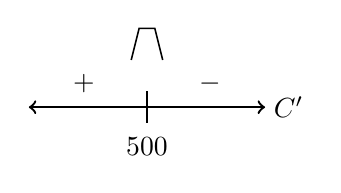
\begin{tikzpicture}[scale=1]
        		\draw[line width=0.03cm,<->] (-1.5,0) -- (1.5,0);
        		\draw[line width=0.02cm] (0,-0.2) -- (0,0.2);
        			\node at (1.8,0) {$C'$};
        		\node at (0,-0.5) {$500$};
        	
        		\node at (-0.8,0.3) {$+$};
        		\node at (0.8,0.3) {$-$};
        	
        		%\draw[line width=0.02cm] (1.3,1) -- (1.4,0.6) -- (1.6,0.6) -- (1.7,1);
        		\draw[line width=0.02cm] (-0.2,0.6) -- (-0.1,1) -- (0.1,1) -- (0.2,0.6);
        		\end{tikzpicture}
		\] \par
	Then $q= 500$ is a maximum. Alternatively, using the fact that $C''(q)= -2$, we know that $C''(150)= -2 < 0$, so that $q= 500$ is a maximum. \pspace
	
	Therefore, the level of production that maximizes the cost of production is $q= 500$.
	\end{enumerate}
}



% Question 6
\newpage
\question[5] Consider the graphs of the functions $f(x)$ and $g(x)$ given below.
	\[
	\fbox{
	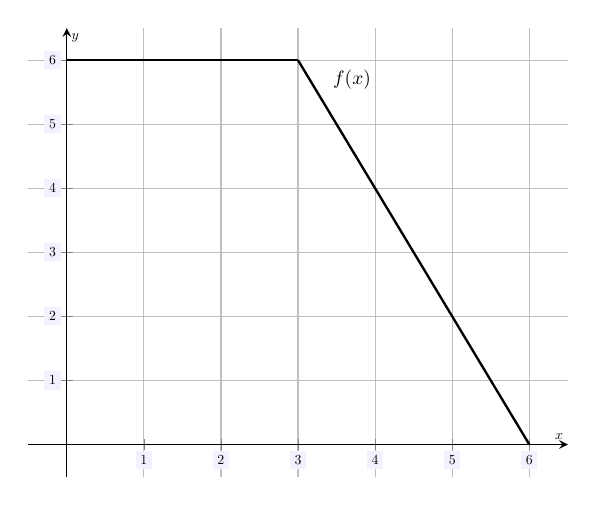
\begin{tikzpicture}[scale=1,every node/.style={scale=0.5}]
	\begin{axis}[
	grid=both,
	axis lines=middle,
	ticklabel style={fill=blue!5!white},
	xmin= -0.5, xmax=6.5,
	ymin= -0.5, ymax=6.5,
	xtick={-1,0,...,6},
	ytick={-1,0,...,6},
	minor tick = {-1,0,...,6},
	xlabel=\(x\),ylabel=\(y\),
	]
	\addplot[line width= 0.03cm,samples=10,domain= 0:3] ({x},{6});
	\addplot[line width= 0.03cm,samples=10,domain= 3:6] ({x},{2*(6 - x)});
	\node at (3.7,5.7) {\scalebox{1.4}{$f(x)$}};
	\end{axis}
	\end{tikzpicture}
	} \hspace{0.5cm}
	\fbox{
	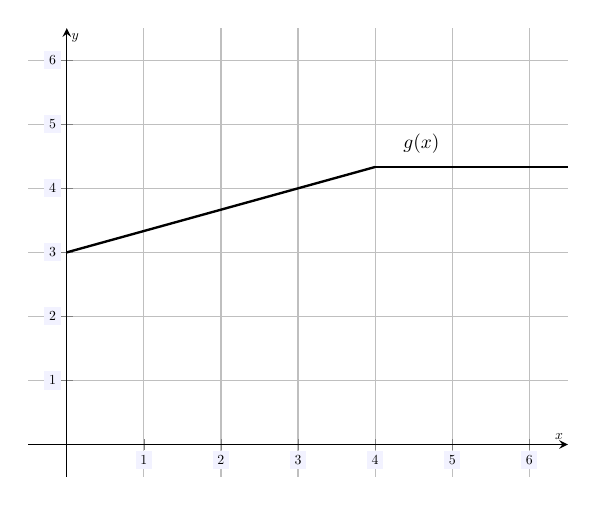
\begin{tikzpicture}[scale=1,every node/.style={scale=0.5}]
	\begin{axis}[
	grid=both,
	axis lines=middle,
	ticklabel style={fill=blue!5!white},
	xmin= -0.5, xmax=6.5,
	ymin= -0.5, ymax=6.5,
	xtick={-1,0,...,6},
	ytick={-1,0,...,6},
	minor tick = {-1,0,...,6},
	xlabel=\(x\),ylabel=\(y\),
	]
	\addplot[line width= 0.03cm,samples=10,domain= 0:4] ({x},{1/3*x + 3});
	\addplot[line width= 0.03cm,samples=10,domain= 4:6.5] ({x},{13/3});
	\node at (4.6,4.7) {\scalebox{1.4}{$g(x)$}};
	\end{axis}
	\end{tikzpicture}
	}
	\]
Based on these plot and showing all your work, compute $\dfrac{d}{dx}\, f \big( g(x) \big) \bigg|_{x=3}$. \pspace

{\itshape Observe that the slope of $f(x)$ at $x= 4$ is $\frac{6 - 0}{3 - 6}= \frac{6}{-3}= -2$ and the slope of $g(x)$ at $x= 3$ is $\frac{3 - 4}{0 - 3}= \frac{-1}{-3}= \frac{1}{3}$. But then\dots
	\[
	\dfrac{d}{dx}\, f \big( g(x) \big) \bigg|_{x=3}= f' \big( g(x) \big) \cdot g'(x) \bigg|_{x=3}= f' \big( g(3) \big) \cdot g'(3)= f'(4) \cdot g'(3)= -2 \cdot \dfrac{1}{3}= -\dfrac{2}{3}
	\]
} \pvspace{0.6cm}



% Question 7
\question[8] Suppose $f(x)$ is a function with $f(10)= -2$, $f'(10)= 8$, and $f''(10)= 12$. 
	\begin{enumerate}[(a)]
	\item Find the tangent line to $f(x)$ at $x= 10$. \pspace
		\[
		\ell(x)= y_0 + m(x - x_0)= f(10) + f'(10) \big(x - 10 \big)= -2 + 8(x - 10)
		\] \pvspace{0.35cm}
	
	\item Use (a) to find an approximation for $f(10.3)$. \pvspace{0.4cm}
		\[
		f(10.3) \approx \ell(10.3)= -2 + 8(10.3 - 10)= -2 + 8(0.3)= -2 + 2.4= 0.4 
		\] \pvspace{0.45cm}
	\item Is your approximation (b) more likely an under-approximation or an over-approximation? Explain. \pspace
	
	{\itshape Because $f''(10)= 12 > 0$, it is likely that (b) is an under-approximation.}
	\end{enumerate}



% Question 8
\newpage
\question[7] Let $f(x)= 2x^2 + 8x - 5$. Using the definition of the derivative, approximate $f'(-1)$. {\itshape While you may check your answer using the derivative shortcuts, you will receive no credit for using derivative shortcuts to find this value.} \pspace

{\itshape \tsol The definition of $f'(a)$ is\dots
	\[
	f'(a):= \lim_{h \to 0} \dfrac{f(a + h) - f(a)}{h}
	\] \par
Here $a= -1$. We choose $h= 0.001$. Then\dots \par
	\[
	\begin{aligned}
	f(a + h)&= f(-1 + 0.001)= f(-0.999)= 2(-0.999)^2 + 8(-0.999) - 5= -10.996 \\[0.3cm]
	f(a)&= f(-1)= 2(-1)^2 + 8(-1) - 5= -11 
	\end{aligned}
	\] \pspace
Therefore, we have\dots
	\[
	f'(1):= \lim_{h \to 0} \dfrac{f(-1 + h) - f(-1)}{h} \approx \dfrac{-10.996 - (-11)}{0.001}= \dfrac{-10.996 + 11}{0.001}= \dfrac{0.004}{0.001}= 4
	\] \vfill

{\small Note. Observe that finding $f'(x)= 4x + 8$, the exact value is $f(-1)= 4(-1) + 8= -4 + 8= 4$.}
}

\end{questions}
\end{document}